\documentclass[a4paper,12pt]{article}
%report, book

%отступы
\usepackage[left=1cm,right=1cm,top=1cm,bottom=2cm,bindingoffset=0cm]{geometry}
\usepackage{indentfirst}

%Рисунки
\usepackage{graphicx}
\usepackage{wrapfig}

%Ссылки
\usepackage{hyperref}
\usepackage[rgb]{xcolor}
\hypersetup{
    colorlinks=true,
    urlcolor=blue
}

%Русский язык
\usepackage[T2A]{fontenc}
\usepackage[utf8]{inputenc}
\usepackage[english,russian]{babel}

%Математика
\usepackage{amsmath,amsfonts,amssymb,amsthm,mathtools}
\usepackage{icomma}

%Доп пакеты
\usepackage{subcaption}
\usepackage{ upgreek }
\usepackage{float}


\usepackage{listings}
\usepackage{xcolor}

\definecolor{codegreen}{rgb}{0,0.6,0}
\definecolor{codegray}{rgb}{0.5,0.5,0.5}
\definecolor{codepurple}{rgb}{0.58,0,0.82}
\definecolor{backcolour}{rgb}{0.95,0.95,0.92}

\lstdefinestyle{mystyle}{
    backgroundcolor=\color{backcolour},   
    commentstyle=\color{codegreen},
    keywordstyle=\color{magenta},
    numberstyle=\tiny\color{codegray},
    stringstyle=\color{codepurple},
    basicstyle=\ttfamily\footnotesize,
    breakatwhitespace=false,         
    breaklines=true,                 
    captionpos=b,                    
    keepspaces=true,                 
    numbers=left,                    
    numbersep=5pt,                  
    showspaces=false,                
    showstringspaces=false,
    showtabs=false,                  
    tabsize=2
}

\lstset{style=mystyle}



%Чтобы найти символ, используем Detexify -> https://detexify.kirelabs.org/classify.html
%Для перевода excel->latex используем Tables Generator -> https://www.tablesgenerator.com/latex_tables
%Для распознования текста по картинке -> https://img2txt.com/ru
%Небольшой тутор по графикам -> http://cs.mipt.ru/python/lessons/lab1.html
%Также -> https://stackoverflow.com/questions/2409774/how-can-i-produce-student-style-graphs-using-matplotlib

%Заголовок
\author{Финоченко Александр}
\title{}
\date{\today}

\begin{document}
\begin{center}
\Large{
\textbf{Лабораторная работа 2}

\textbf{Сортировки}

Финоченко Александр Викторович Б02-201
}

\end{center}
\large

\textbf{Цель работы:} написать улучшения к сортировкам с квадратичной асимптотической сложностью, провести декомпозицию на элементарные шаги и
протестировать отдельные функции.

\section*{Шейкерская сортировка}
Ниже приведены функции прямого прохода, обратного прохода и шейкерской сортировки.

\begin{lstlisting}[language=C++]
bool forward_step(U arr[], U const begin_idx, U const end_idx) {
    bool sorted = true;
    for (U idx = begin_idx; idx != end_idx; ++idx) {
        if (arr[idx] > arr[idx + 1]) {
            auto tmp = arr[idx];
            arr[idx] = arr[idx + 1];
            arr[idx + 1] = tmp;
            sorted = false;
        }
    }
    return sorted;
}

bool backward_step(U arr[], U const begin_idx, U const end_idx) {
    bool sorted = true;
    for (U idx = end_idx - 1; idx != begin_idx - 1; --idx) {
        if (arr[idx] > arr[idx + 1]) {
            auto tmp = arr[idx];
            arr[idx] = arr[idx + 1];
            arr[idx + 1] = tmp;
            sorted = false;
        }
    }
    return sorted;
}

void shaker_sort(U arr[], U const begin_idx, U const end_idx) {
    bool sorted = false;
    while (!sorted) {
        sorted = forward_step(arr, begin_idx, end_idx);
        sorted = backward_step(arr, begin_idx, end_idx);
        assert(is_sorted(arr, begin_idx, end_idx));
    }
}
\end{lstlisting}

Проверка того, что массив отсортирован, производилась с помощью функции is\_sorted:

\begin{lstlisting}[language=C++]
template <typename T>
bool is_sorted(T arr[], U const begin_idx, U const end_idx) {
    bool sorted = true;
    for (U idx = begin_idx; idx != end_idx; idx++) {
        if (arr[idx] > arr[idx + 1])
            sorted = false;
    }
    return sorted;
}
\end{lstlisting}

Программа успешно отработала, что означает, что функция сортировки работает нормально.



\section*{Сортировка расчёской}

Сортировка проводится сначала по $N/4$ и $N/2$, далее проводится обычная сортировка пузырьком. Полный код функции сортировки расчёской представлен ниже

\begin{lstlisting}[language=C++]
template <typename T>
bool is_N4_sorted(T arr[], U const begin_idx, U const end_idx) {
    U step = (end_idx - begin_idx + 1) / 4;
    bool sorted = true;
    for (U idx = begin_idx; idx + step <= end_idx; idx += step) {
        if (arr[idx] > arr[idx + step])
            sorted = false;
    }
    return sorted;
}

template <typename T>
bool is_N2_sorted(T arr[], U const begin_idx, U const end_idx) {
    U step = (end_idx - begin_idx + 1) / 2;
    bool sorted = true;
    for (U idx = begin_idx; idx + step <= end_idx; idx += step) {
        if (arr[idx] > arr[idx + step])
            sorted = false;
    }
    return sorted;
}

ULL N4_sort(U arr[], U const begin_idx, U const end_idx) {
    U step = (end_idx - begin_idx + 1) / 4;
    ULL count = 0;
    bool sorted = false;
    while (!sorted) {
        sorted = true;
        for (U idx = begin_idx; idx + step <= end_idx; idx += step) {
            if (arr[idx] > arr[idx + step]) {
                auto tmp = arr[idx];
                arr[idx] = arr[idx + step];
                arr[idx + step] = tmp;
                sorted = false;
                count++;
            }
        }
    }
    assert(is_N4_sorted(arr, begin_idx, end_idx));
    return count;
}

ULL N2_sort(U arr[], U const begin_idx, U const end_idx) {
    U step = (end_idx - begin_idx + 1) / 2;
    ULL count = 0;
    bool sorted = false;
    while (!sorted) {
        sorted = true;
        for (U idx = begin_idx; idx + step <= end_idx; idx += step) {
            if (arr[idx] > arr[idx + step]) {
                auto tmp = arr[idx];
                arr[idx] = arr[idx + step];
                arr[idx + step] = tmp;
                sorted = false;
                count++;
            }
        }
    }
    assert(is_N2_sorted(arr, begin_idx, end_idx));
    return count;
}

ULL comb_sort(U arr[], U const begin_idx, U const end_idx) {
    ULL count1 = N4_sort(arr, begin_idx, end_idx);
    ULL count2 = N2_sort(arr, begin_idx, end_idx);
    ULL count = 0;

    bool sorted = false;
    while (!sorted) {
        sorted = true;
        for (U idx = begin_idx; idx != end_idx; ++idx) {
            if (arr[idx] > arr[idx + 1]) {
                auto tmp = arr[idx];
                arr[idx] = arr[idx + 1];
                arr[idx + 1] = tmp;
                sorted = false;
                count++;
            }
        }
    }
    return count1 + count2 + count;
}
\end{lstlisting}

Программа была проверена на случайно сгенерированных массивах и ошибок не выдавала.
Сама функция одновременно сортирует массив и подсчитывает количество перестановок.

Далее представлен график зависимости времени и числа перестановок в зависимости от количества элементов $N$

\begin{center}
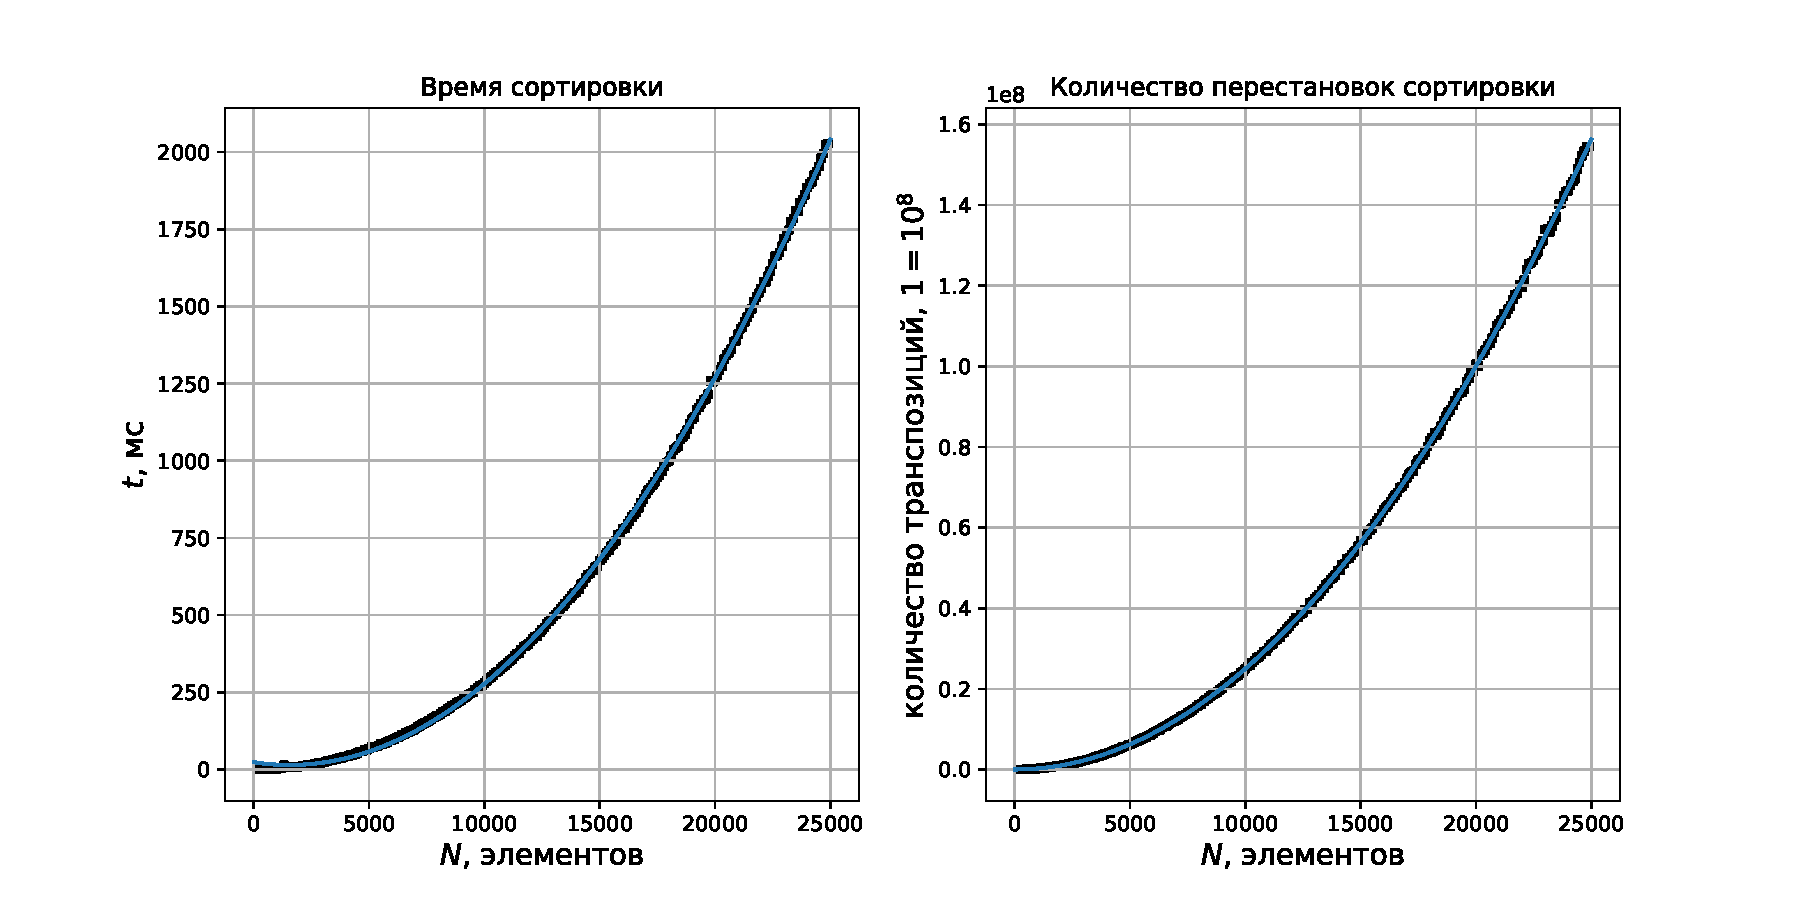
\includegraphics[scale=0.6]{Figure_1.pdf}
\end{center}

Видно, что зависимость квадратичная.

\section*{Сортировка Шелла}
Общая функция для сортировки Шелла с некоторым шагом
\begin{lstlisting}
ULL shell_sort_i(U arr[], U const begin_idx, U const end_idx, U step) {
    ULL count = 0;
    if (begin_idx + step > end_idx)
        return 0;
    for (int last = end_idx - step; last >= 0; last -= step) {
        auto tmp_idx = last;
        while (tmp_idx + step <= end_idx && arr[tmp_idx] > arr[tmp_idx + step]) {
            auto tmp = arr[tmp_idx];
            arr[tmp_idx] = arr[tmp_idx + step];
            arr[tmp_idx + step] = tmp;
            tmp_idx += step;
            count++;
        }
    }
    return count;
}
\end{lstlisting}

\subsection*{Последовательность $d_{i+1} = d_i / 2, d_1 = N$}
Для шага $d_{i+1} = d_i / 2, d_1 = N$ функция сортировки Шелла выглядит так
\begin{lstlisting}
ULL shell_sort(U arr[], U const begin_idx, U const end_idx) {
    ULL count = 0;
    U step = (end_idx - begin_idx + 1);

    while (step != 0) {
        count += shell_sort_i(arr, begin_idx, end_idx, step);
        step /= 2;
    }
    return count;
}
\end{lstlisting}

Предполагая, что при больших $N$ время работы программы приближается к $N^{\alpha}$, определим это $\alpha$. Для этого перейдём к логарифмам, тогда $\ln t = \alpha \ln N$. Получаем, что $\alpha = 1.96$

\begin{center}
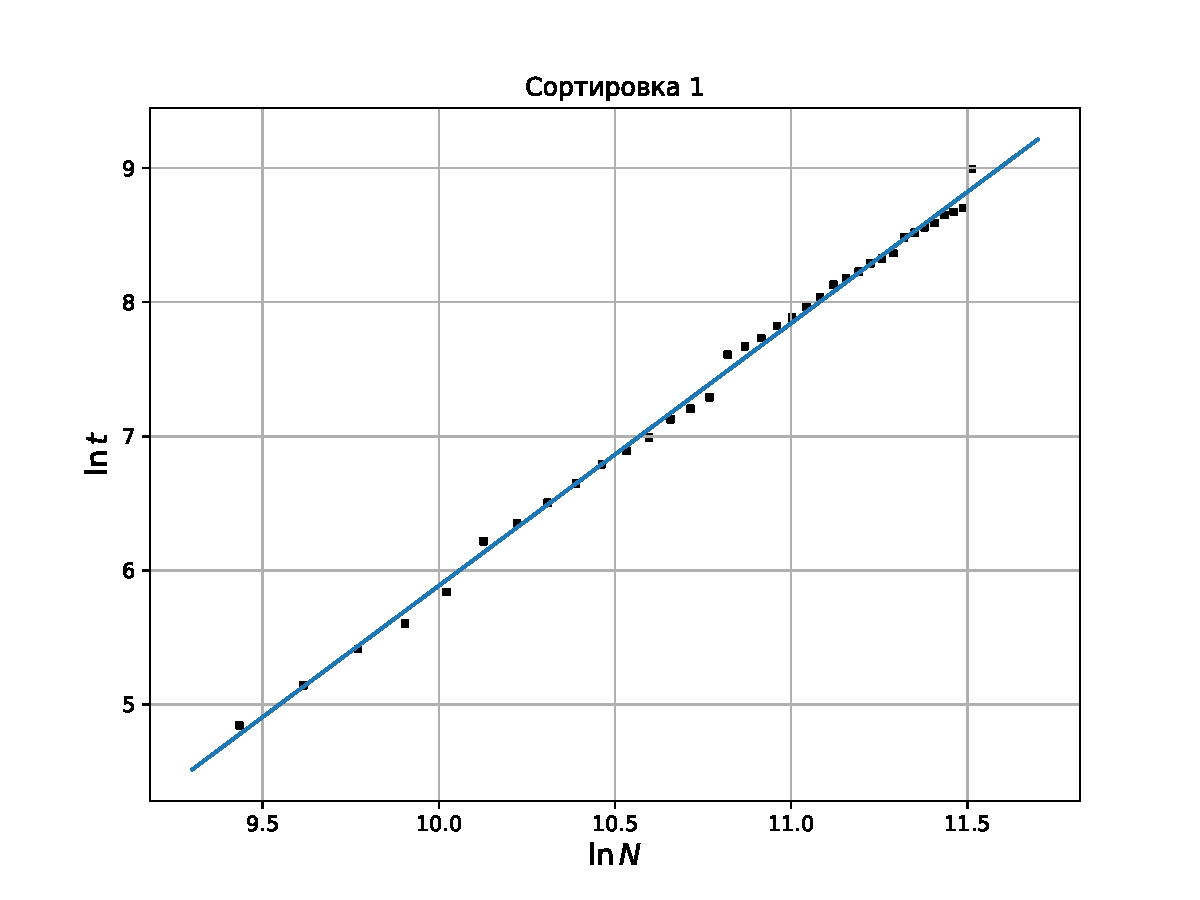
\includegraphics[scale=0.6]{Figure_2.pdf}
\end{center}

Среднее количество перестановок равно $6.88 \cdot 10^8$.

\subsection*{Последовательности Хиббарда}
Проделаем тоже самое. Функция функция сортировки Шелла выглядит так
\begin{lstlisting}
ULL shell_sort(U arr[], U const begin_idx, U const end_idx) {
    ULL count = 0;
    U i = 0;
    while ((U)pow(2, i) - 1 <= (end_idx - begin_idx + 1)) {
        ++i;
    } 
    --i;
    U step = (U) pow(2, i) - 1;
    while (step != 0) {
        count += shell_sort_i(arr, begin_idx, end_idx, step);
        i--;
        step = pow(2, i) - 1;
    }
    return count;
}
\end{lstlisting}

Если $\ln t = \alpha \ln N$, то $\alpha = 1.99$


\begin{center}
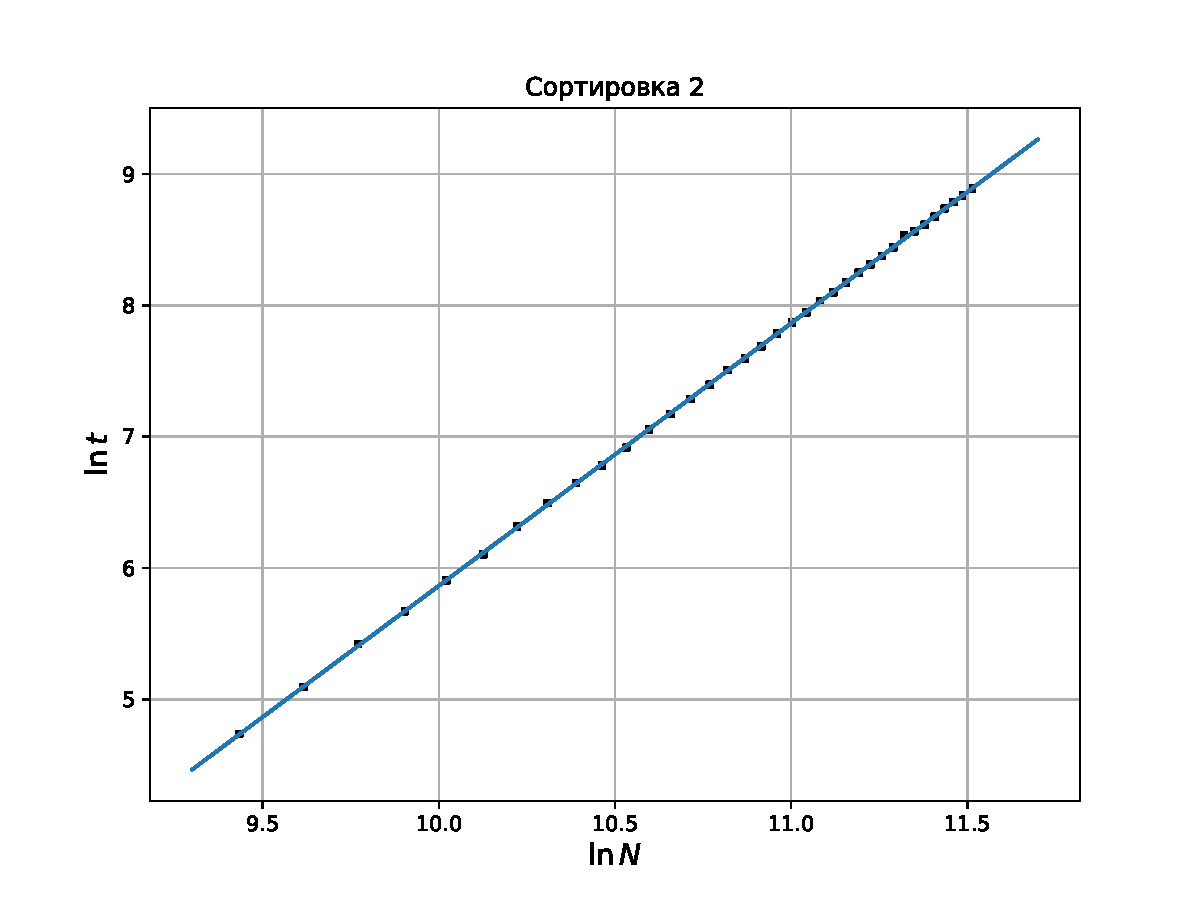
\includegraphics[scale=0.6]{Figure_3.pdf}
\end{center}

Среднее количество перестановок равно $7.06 \cdot 10^8$.

\subsection*{Обратная последовательность Фибоначчи}
Для обратной последовательности Фибоначчи функция сортировки Шелла выглядит так

\begin{lstlisting}
ULL shell_sort(U arr[], U const begin_idx, U const end_idx) {
    ULL count = 0;
    vector<U> f_arr = fib_arr(end_idx - begin_idx + 1);
    U step;
    for (U i = size(f_arr) - 1; i != 1; i--) {
        step = f_arr[i];
        count += shell_sort_i(arr, begin_idx, end_idx, step);
    }
    return count;
}
\end{lstlisting}

Здесь проше использовать векторы. Функция fib\_arr нужна, чтобы быстро находить числа Фибоначчи

\begin{lstlisting}
vector<U> fib_arr(U N) {
    U F_0 = 0; U F_1 = 1;
    U n = 0;
    while (F_1 <= N) {
        U temp = F_1;
        F_1 += F_0;
        F_0 = temp;
        n++;
    }
    F_0 = 0; F_1 = 1;
    vector<U> fib_arr(n + 1);
    fib_arr[0] = 0;
    for (U i = 1; i <= n; i++) {
        fib_arr[i] = F_1;
        U temp = F_1;
        F_1 += F_0;
        F_0 = temp;
    }
    return fib_arr;
}
\end{lstlisting}


Если $\ln t = \alpha \ln N$, то $\alpha = 1.99$


\begin{center}
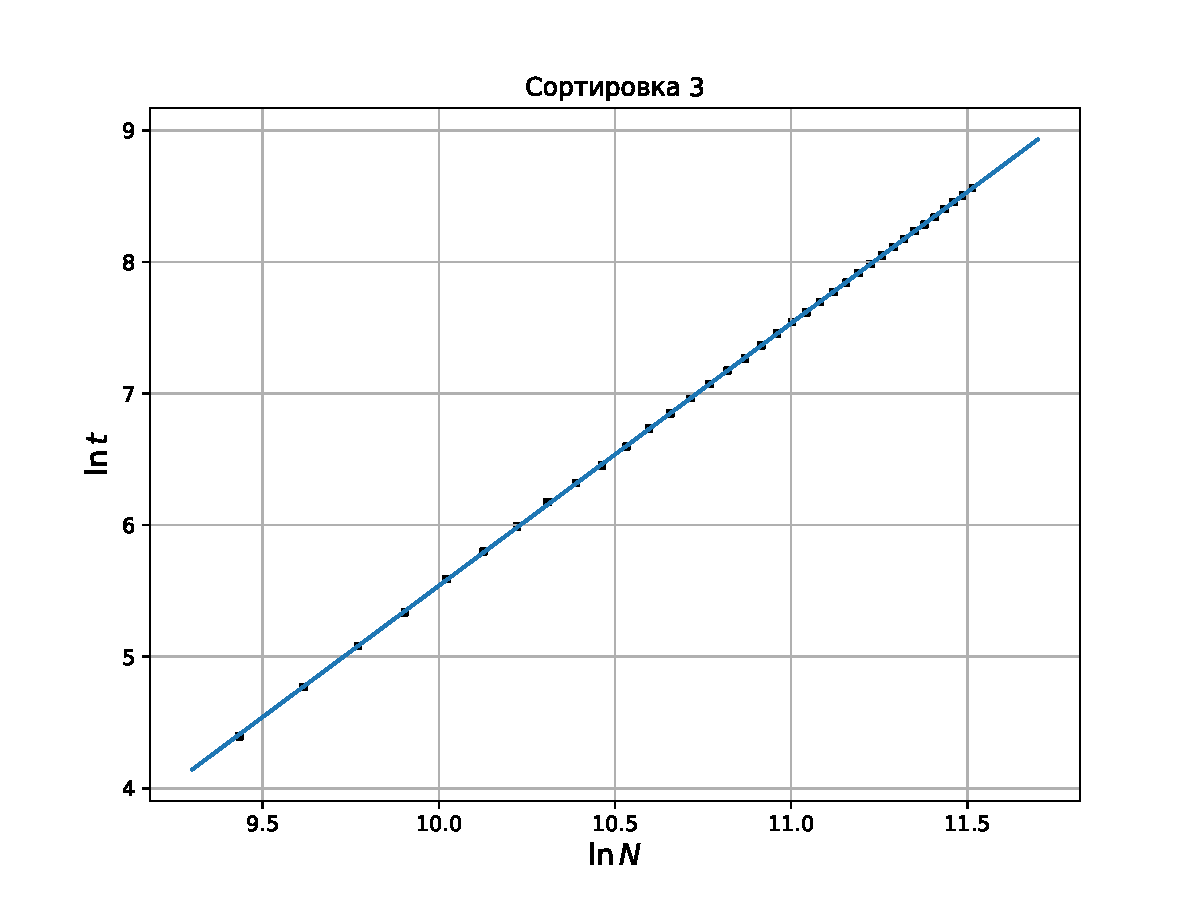
\includegraphics[scale=0.6]{Figure_4.pdf}
\end{center}

Среднее количество перестановок равно $5.07 \cdot 10^8$.

\subsection*{Вывод}
Получаем, что наиболее эффективная по времени является 1 последовательность, наиболее эффективная по числу перестановок - 2 последовательность.














\end{document}